\documentclass[aip,jcp,reprint,floatfix]{revtex4-1}

\usepackage{amsmath,amssymb}
\usepackage{epsfig}
\usepackage{graphicx}
\usepackage{dcolumn}
\usepackage{bbold}
\usepackage{natbib}
\usepackage[normalem]{ulem} % to strike out plain text
\usepackage[colorlinks=true,citecolor={blue},urlcolor={blue}, linkcolor=blue]{hyperref}%
\usepackage[utf8]{inputenc}
\usepackage{amsthm}
\usepackage{braket}
\usepackage{verbatim}
\usepackage{mdframed}


\begin{document}


\title{Quantum Mechanical Many-body Problems with Machine Learning Algorithms}


\author{Scott Bogner}
\affiliation{National Superconducting Cyclotron Laboratory and Department of Physics and Astronomy, Michigan State University, East Lansing, MI 48824, USA}

\author{Morten Hjorth-Jensen}
\affiliation{National Superconducting Cyclotron Laboratory and Department of Physics and Astronomy, Michigan State University, East Lansing, MI 48824, USA}
\affiliation{Department of Physics and Center for Computing in Science Education, University of Oslo, N-0316 Oslo, Norway}


\maketitle

\section{Introduction and motivation}

Traditional many-body methods like full configuration interaction
theory (FCI), coupled-cluster (CC) theory, many-body perturbation theory (MBPT),
in-medium similarity renormalization group (IMSRG),
various Monte Carlo methods and many other many-body
approaches, have been rather successful in describing properties of
interacting many-body systems. These methods have been widely used in
condensed matter physics, nuclear physics, quantum chemistry and
materials science, just to mention a few of the areas of
applicability.

However, essentially all of these methods face what is
normally called the curse of dimensionality. For wave function based
method like FCI or CC theories where the original continuous problem
is discretized in terms selected basis functions and/or many-body
excitations, the dimensionality of the systems under study grows almost
exponentially when larger basis sets and/or number of particles are
included. As an example, nuclear physics 
systems close to the limits of stability pose in
particular a tough problem to many-body practitioners in terms of a dramaticn
increase of the number of relevant degrees of freedom. To describe say
weakly bound nuclei within the framework of a wave function based
approach, requires often a single-particle basis which includes bound,
weakly bound and unbound states, increasing thereby considerably the
number of many-body basis states. This renders often a standard
FCI calculation infeasible. Within the above mentioned
many-body methods there are however several interesting theoretical
approachs which attempt at circumventing the dimensionality
curse. Smarter basis sets is one of these approaches, as well as the
resummation of specific correlations and the recently proposed
stochastic sampling of many-body states in both FCI and CC
calculations.

Recently, several authors have pointed to  possibilities within the
broad fields of Machine Learning and Quantum Computing as approaches
that hold great promise in tackling the ever increasing
dimensionalities. There are several groups worldwide which now focus
on Machine Learning and/or Quantum Computing applied to many-body
problems.
Machine learning (ML) is an extremely rich field, in spite of its
young age. The increases we have seen during the last three decades in
computational capabilities have been followed by developments of
methods and techniques for analyzing and handling large date sets,
relying heavily on statistics, computer science and mathematics.  The
field is rather new and developing rapidly.

Machine Learning based methods offer several possibilities to
circumvent the abovementioned dimensionality problems, as well as
allowing us to model quantum mechanical systems with less a priori
knowlegde. For complex many-body systems like those which arise in
nuclear physics (in particular with the increase in the number of
degrees of freedom for nuclei close to their limits of stability).

We have recently started to explore several approaches based on deep
learning algorithms, with an emphasis on neural networks and so-called
Boltzmann machines, with several promising results for interacting
many-fermion systems, see some of the results below. Our applications
so far have been to systems of electrons confined to move in two or
three-dimensional regions (so-called quantum dots) and systems of
bosons (weakly and strongly interacting) using a mix of neural network
based algorithms and variational quantum Monte Carlo approaches.
Furthermore, we have also explored the solution of the Similarity
Renormalization Group set of equations using deep learning algorithms.


\section{Opportunities, challenges and new advances}

Neural-network quantum states (NQS) are a representation of the many-body
wave-function in terms of artificial neural networks (ANNs).
A commonly adopted choice is to parameterize
wave-function amplitudes as a feed-forward neural network.


One of the specific challenges emerging in the quantum domain is
imposing physical symmetries in the NQS representations. In the case
of a periodic arrangement of matter (often used in the simulation of
infinite systems like nuclear matter and the homogeneous electron
gas), spatial symmetries can be imposed using convolutional
architectures similar to what is used in image classification tasks.
While spatial symmetries have analogous counterparts in other ML
applications, satisfying more involved quantum symmetries often needs
a deep rethinking of ANN architectures.  The most notable case in this
sense is the \emph{exchange symmetry}.  For bosons, this amounts to
imposing the wave-function to be permutationally invariant with
respect to exchange of particle indices. The Bose-Hubbard model has
been adopted as a benchmark for ANN bosonic architectures, with
state-of-the-art results having been obtained.  The most challenging
symmetry is, however, certainly the fermionic one.  In this case, the
NQS representation needs to encode the antisymmetry of the
wave-function (exchanging two particle positions, for example, leads
to a minus sign). In this case, different approaches have been
explored, mostly expanding on existing variational ansatz for
fermions. We have for example explicitely included the fermion
antisymmetry by multiplying the NQS with an explicit Slater
determinant.  The situation for fermions is certainly the most
challenging for ML approaches at the moment, owing to the specific
nature of the symmetry.  On the applications side, NQS representations
have been used so-far along three main different research lines. These
are:

\begin{enumerate}
\item Representation of states: An active area of research concerns the general expressive power
of NQS, as also compared to other families of variational states.
Theoretical activity on the representation properties
of NQS seeks to understand how large, and how deep
should be neural networks describing interesting interacting quantum systems.
\item Learning from data: Parallel to the activity on understanding the theoretical properties of NQS,
a family of studies in this field is concerned with the
problem of understanding how hard it is, in practice, to learn
a quantum state from numerical data.
This can be realized using either synthetic data (for example coming from numerical simulations)
or directly from experiments.

This line of research has been explored in the supervised learning setting, to
understand how well NQS can represent states that are not easily expressed (in closed analytic form) as ANN.
The goal is then to train a NQS network to represent, as close as possible, a certain target state
whose amplitudes can be efficiently computed.
\item Finally, one of the main applications for the NQS representations is in the context
of variational approximations for many-body quantum problems.
The goal of these approaches is, for example, to approximately solve the Schr\"{o}dinger equation using a NQS representation for the wave-function.
In this case, the problem of finding the ground state of a given quantum Hamiltonian $H$ is formulated in variational terms as the problem of learning NQS weights $W$
minimizing $E(W)=\langle\Psi(W)|H|\Psi(W)\rangle/\langle\Psi(W)|\Psi(W)\rangle$. This is achieved using a learning scheme based on variational
Monte Carlo optimization.
Within this family of applications,
no external data representative of the quantum state is given, thus they typically demand a larger computational burden than supervised and unsupervised learning schemes for NQS.
\end{enumerate}


We have worked on the latter approach in connection with studies of
quantum dot systems (confined two-dimensional and three-dimensional
electron systems).  Using Quantum Monte Carlo samplings (QMC), a
practical issue often resulting is that of providing efficient
sampling schemes of high-dimensional spaces (path integrals,
perturbation series, etc..). This requires a careful tuning which is often
problem-dependent.  Devising general-purpose samplers for these
representations is therefore a particularly challenging
problem. Unsupervised ML methods can, however, be adopted as a tool to
speed-up Monte Carlo sampling for both classical and quantum
applications. In the figure here, we show the speed-up obtained when
using Restricted Boltzmann machines (RBM) for systems of
two-dimensional quantum dots (with $N=2,6,12,20,30,42,56,72$
electrons) compared with a Variational Monte Carlo calculation
(VMC). The results for the energies are similar. The main speed-up is
due to a simpler mathematical form for the correlated part of the
trial wave function. In the RBM calculation we used a simple Slater
determinant for the electrons using Hermite polynomials only. However,
the results for energies and other observables can be improved upon by
multiplying the NQS with a Jastrow factor (RBM+PJ/SJ). This leads
however to an increase in CPU time  since the number of parameters to optmize
increases. How to speed up the calculation of the Jastrow factor is
also an important issue.
\begin{figure}[hbtp]
        \centering
        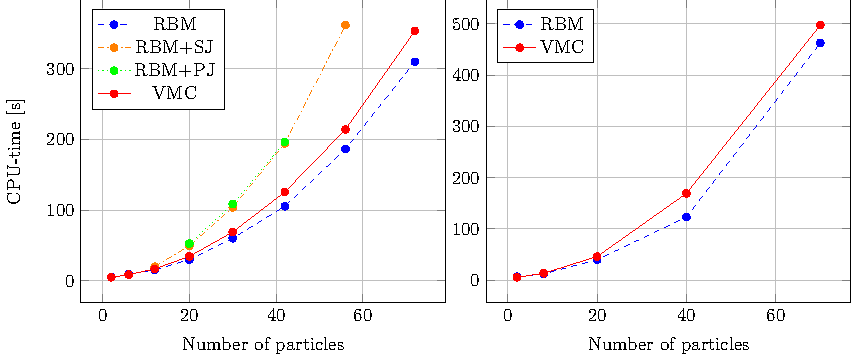
\includegraphics[scale=0.5]{fig1.pdf}
        \caption{Speed-up obtained when
using Restricted Boltzmann machines (RBM) for systems of
two-dimensional quantum dots (with $N=2,6,12,20,30,42,56,72$
electrons) compared with a Variational Monte Carlo calculation
(VMC). The results for the energies are similar. The main speed-up is
due to a simpler mathematical form for the correlated part of the
trial wave function. In the RBM calculation we used a simple Slater
determinant for the electrons using Hermite polynomials only. However,
the results for energies and other observables can be improved upon by
multiplying the NQS with a Jastrow factor (RBM+PJ/SJ).}
\end{figure}


While exact for a large family of bosonic and fermionic systems, QMC techniques
typically incur in a severe sign problem when dealing with several
interesting fermionic models, as well as frustrated spin Hamiltonians.
In this case, it is tempting to use ML approaches to attempt a direct
or indirect reduction of the sign problem. While only in its first
stages, this family of applications has been used to infer information
about fermionic phases through hidden information in the Green's function.

Similarly, ML techniques can help reduce the burden of more subtle
manifestations of the sign problem in dynamical properties of quantum
models. In particular, the problem of reconstructing spectral functions
from imaginary-time correlations in imaginary time is also a field
in which ML can be used as an alternative to traditional maximum-entropy
techniques to perform analytical continuations of QMC data.

Applications of ML to quantum many-body problems have seen a fast-pace
progress in the past few years, touching a diverse selection of topics
ranging from numerical simulation to data analysis. The potential of
ML techniques has already surfaced in this context, already showing
improved performance with respect to existing techniques on selected
problems. To a large extent, however, the real power of ML techniques
in this domain has been only partially demonstrated, and several open
problems remain to be addressed.
In the context of variational studies with NQS, for example, the
origin of the empirical success obtained so far with different kind of
neural network quantum states is not equally well understood as for
other families of variational states, like tensor networks. Key open
challenges remain also with the representation and simulation of
fermionic systems, for which efficient neural-network representation
are still to be found.


Tensor-network representations for ML purposes, as well as
complex-valued networks like those used for NQS, play an important
role to bridge the field back to the arena of computer
science. Challenges for the future of this research direction consist
in effectively interfacing with the computer-science community, while
retaining the interests and the generality of the physics tools.


We have been able recently to study both interacting bosonic systems
and interacting fermionic systems (electrons confined to two- or
three-dimensional regions). We are planning to extend our applications to studies of infinite systems
like the homogeneous electron gas.  We plan also to address several of the
above issues in the next few years (a three to five year perspective).
The real challenge however is to extend these studies to nuclear
systems. Applying ML methods to nuclear systems based on the above
approaches is our central goal for the next five to ten years.

\end{document}









